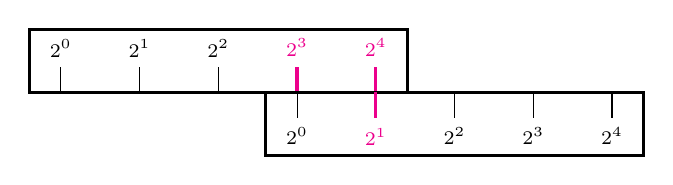
\begin{tikzpicture}[x=4cm, y=4cm, every node/.style={font=\scriptsize}]
\draw[very thick] (-0.1,0) rectangle (1.1,0.2);
\foreach \i in {0, 1, 2}
	\draw (\i*0.25,0) -- ++(0,0.08) node[above] {$2^{\i}$};
\foreach \i in {3, 4}
	\draw[magenta, very thick] (\i*0.25,0) -- ++(0,0.08) node[above] {$2^{\i}$};
% dolna linijka
\begin{scope}[shift={(0.75,0)}]
\draw[very thick] (-0.1,0) rectangle (1.1,-0.2);
\foreach \i in {0, 2, 3, 4}
	\draw (\i*0.25,0) -- ++(0,-0.08) node[below] {$2^{\i}$};
\foreach \i in {1}
	\draw[magenta, very thick] (\i*0.25,0) -- ++(0,-0.08) node[below] {$2^{\i}$};
\end{scope}
\end{tikzpicture}